\chapter{TacOSのセマフォ}
\label{tacosImpSemaphore}
TacOSではプロセス同期の基本機構としてセマフォを用いる.
セマフォ機構はマイクロカーネルが提供する.
今のところTacOSでセマフォを利用できるのは,
カーネルモードで実行されるサーバプロセスとマイクロカーネルだけである.

%==============================================================================
\section{データ構造}
セマフォはリスト\ref{tacosStructSem}に示す構造体である\footnote{
  \url{https://github.com/tctsigemura/TacOS/blob/master/os/kernel/process.hmm}
  の一部である.}.
また,\figref{tacosSemaphore}にセマフォ関連データの構造を示す.
\|semTbl|はセマフォの一覧である.
システム起動時に\|SEM_MAX|個(30個)のセマフォを準備し\|semTbl|に登録する.
\|semInUse|はセマフォが使用中かどうかを記録する論理型の配列である.
セマフォが必要になった時に,一覧の中から空きセマフォを選んで使用する.
セマフォは一覧のインデクス(\emph{セマフォ番号})で識別するので,
P操作やV操作を行う関数の引数がセマフォ番号になる.

\lstinputlisting[numbers=none,float=btp,label=tacosStructSem,
  firstline=99,lastline=104,
  caption=TacOSのセマフォ構造体]{TacOS/kernel/process.hmm}

\begin{myfig}{btp}{TacOSのセマフォ関連データ構造}{tacosSemaphore}
  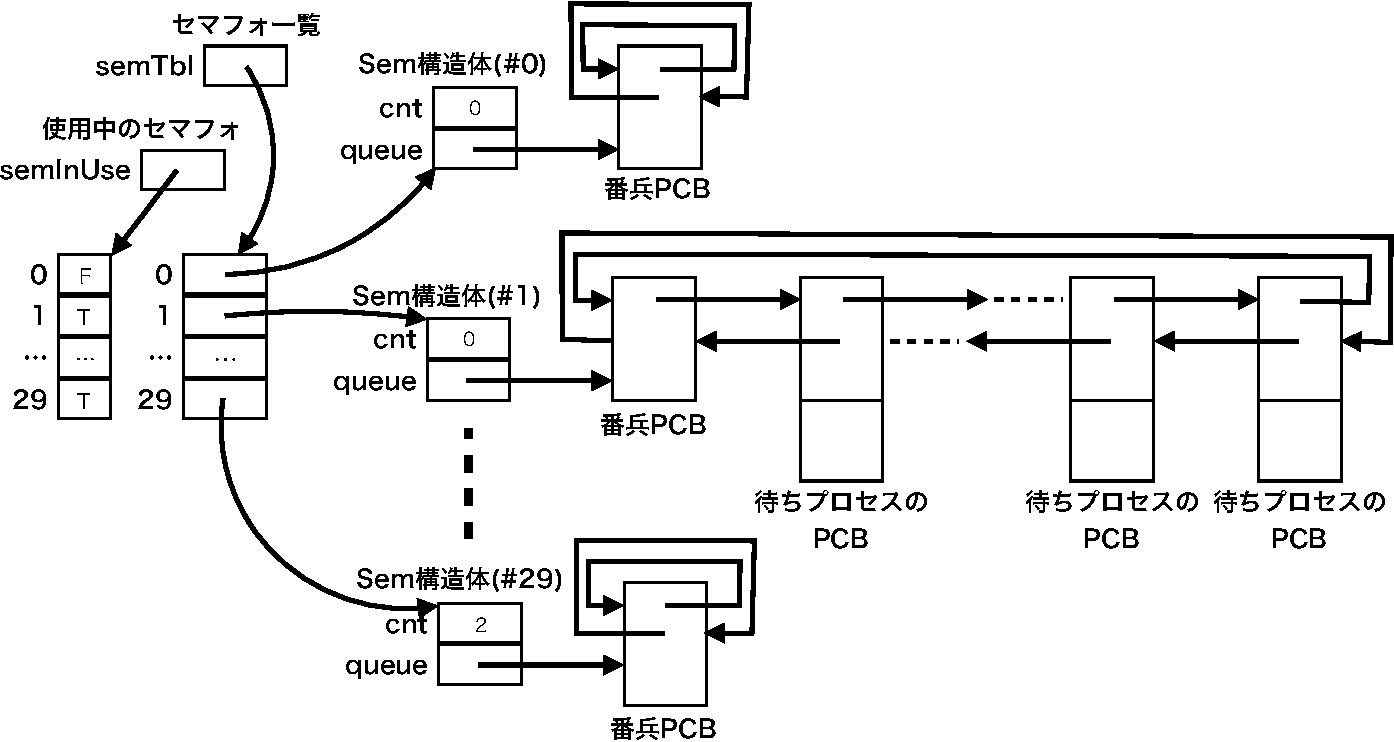
\includegraphics[scale=0.66]{Fig/tacosSemaphore-crop.pdf}
\end{myfig}

セマフォ構造体(\|Sem|構造体型)は,
セマフォの値(\|cnt|)とプロセスの待ち行列(\|queue|)を持っている.
\|cnt|はカウンタなので,TacOSのセマフォはカウンティングセマフォである.
セマフォの数は30個に固定されており,
システム起動時に\|Sem|構造体と番兵PCBで初期化される.
プロセスの待ち行列はPCBの双方向循環リストとして表現される.
待ち行列は到着順にソートされるので,
セマフォ待ちプロセスは\emph{FIFO方式のスケジューリング}を受ける.
次に,\figref{tacosSemaphore}で表している三つのセマフォについて説明する.

\begin{description}
\item [Sem構造体(\#0)]
  セマフォ一覧(\|semTbl|)の第0行に登録されている.
  Sem構造体(\#0)は使用されていないSem構造体を表している.
  \|semInUse|の対応する要素はFalseになっている.

\item [Sem構造体(\#1)]
  値が0の時に複数のプロセスがP操作を行った状態である.
  使用中なので\|semInUse|の対応する要素はTrueになっている.
  P操作を行いブロックしたプロセスがセマフォの待ち行列に入っている.
  プロセスは待ち行列の最後(図では右)に追加され,
  待ち行列の先頭(図では左)から取り出される.
  同じセマフォについて,プロセスはFCFSのスケジューリングが適用される.

\item [Sem構造体(\#29)]
  V操作の結果,値が2になっている状態を表している.
  使用中なので\|semInUse|の対応する要素はTrueになっている.
  値が1以上の時は,待ち行列が必ず空になる.
\end{description}

%==============================================================================
\section{使用例}
リスト\ref{tacosSemUse}にセマフォの使用例を示す.
これは,リスト\ref{semMutex}をTacOS用に書き換えたものである.

\lstinputlisting[numbers=left,float=btp,label=tacosSemUse,
  caption=TacOSでのセマフォの架空の使用例]{TacOS/samples/tacosSemUse.cmm}

\begin{description}
\item [共有変数と相互排除用のセマフォ]
  以前の例ではセマフォを\|Semaphore|型の変数として扱っていた.
  今回の例ではセマフォを番号で指定するようになっている.
  そのため3行は,
  セマフォ型変数の宣言から番号を記憶する整数型変数の宣言に変更された.
\item [使用するセマフォの割当て]
  セマフォはマイクロカーネル内部で
  \figref{tacosSemaphore}に示したように管理されている.
  4行のプロセスの初期化ルーチン\|initProc()|中で,
  マイクロカーネルが提供する\|newSem()|関数を用いてセマフォの割当てを受ける.
  \|newSem()|関数の引数はセマフォの初期値である.
\item [P操作とV操作]
  P操作関数は\|semP()|,V操作関数は\|semV()|である.
  10行,12行,18行,20行のようにセマフォ番号を引数に使用する.
\end{description}

%==============================================================================
\section{割当}
リスト\ref{tacosNewSem}にセマフォ割当と解放ルーチンを示す\footnote{
  \url{https://github.com/tctsigemura/TacOS/blob/master/os/kernel/kernel.cmm}
  の一部である.}.

\lstinputlisting[numbers=left,float=btp,label=tacosNewSem,
  firstline=142,lastline=164,
  caption=TacOSのセマフォ割当て解放ルーチン]{TacOS/kernel/kernel.cmm}

\begin{description}
\item [データ構造]
  1行の\|semTbl|,2行の\|semInUse|は,
  \figref{tacosSemaphore} に描かれている「セマフォ一覧」と
 「使用中のセマフォ」のことである.
 \|semTbl|はTacOSの起動時に「Sem構造体」や「番兵PCB」で初期化される.

\item [割込み禁止による相互排除]
  5行の\|newSem()|関数が\|semTbl|から未使用のセマフォを探す.
  \|newSem()|関数や後述の\|semP()|,\|semV()|関数は,
  複数のプロセスから並列に呼び出され\|semTbl|や\|semInUse|をアクセスする.
  これらのデータ構造はプロセス間の共有データである.
  \|newSem()|関数の内部はこれら共有データのクリティカルセクションに当たるので
  相互排他が必要である.
  TaCはシングルプロセッサシステムなので,
  \ref{disableInterrupt}で紹介した「割込み禁止による相互排除」を行う.

  6行では,
  現在のフラグ\footnote{CPUのPSWのフラグのこと.}の値を\|r|に保存した後,
  「割込み禁止(\|DI|)」にしている.
  \|setPri()|関数はフラグの値を読み出し,
  同時に引数値をフラグにセットするアセンブリ言語ルーチンである\footnote{
    \texttt{setPri()}関数の詳細は「\ref{setPri} \texttt{setPri()}関数」を
    参照のこと}.
  \|newSem()|関数はカーネルモードで呼び出すので,
  実行モードが変化しないように「カーネルモード(\|KERN|)」も指定している.

  7行からのループで使用されていないセマフォを探す.
  割込み禁止で実行するので探索の途中でプリエンプションは発生しない.
  未使用のセマフォが見つかったら12行でそれの番号を返す.

  クリティカルセクションが終わるので,通常は割込みを許可するが,
  \|newSem()|関数を呼び出す前から割込み禁止だった場合もある.
  11行では6行で保存した\|r|を用いてフラグの状態を復旧している.
  もともと\|newSem()|関数が割込み許可状態で呼び出された場合だけ
  割込み許可状態に戻る.

\item [エラー処理]
  未使用のセマフォが見つからなかった場合は,15行で\|panic()|関数を呼び出す.
  現在のTacOSでは,
  セマフォを使用できるのはマイクロカーネルとサーバプロセスだけである.
  セマフォが不足するようならオペレーティングシステムのバグである.
  \|panic()|関数はエラーメッセージを表示した後,CPUを停止する.
  \|panic()|関数は戻ってこないので16行は実行されない.

\item [解放ルーチン]
  21行の\|freeSem()|は割当てられていたセマフォを解放する.
  共有変数\|semInUse|配列の書き換えは,
  単一のストア機械語命令で終了するので割込み禁止にする必要はない\footnote{
    CPUが機械語命令の途中で割込みを受け付けることはない.}.
\end{description}

%==============================================================================
\section{P操作ルーチン}
リスト\ref{tacosSemP}にP操作ルーチンを示す\footnote{
  \url{https://github.com/tctsigemura/TacOS/blob/master/os/kernel/kernel.cmm}
  の一部である.}.
P操作ルールーチンは\|semP()|関数のことである.

\lstinputlisting[numbers=left,float=btp,label=tacosSemP,
  firstline=171,lastline=186,
    caption=TacOSのP操作ルーチン]{TacOS/kernel/kernel.cmm}

\begin{description}
\item [割込み禁止による相互排除]
  \|semP()|関数も,\|semInUse|や,\|semTbl|の配下のSem構造体,
  PCB構造体等の共有データをアクセスするので相互排除を必要とする.
  \|semP()|関数の内部は2行と15行の\|setPri()|関数を用いて,
  割込み禁止による相互排除を行っている.

\item [セマフォ番号からセマフォ構造体への変換]
  3行で引数のセマフォ番号が正当なものかチェックしている.
  不正なものが渡されるようならオペレーティングシステムのバグなので
  \|panic()|関数を用いてシステムを停止させる.
  セマフォ番号が正しい場合は,
  6行で\|semTbl|配列から目的のセマフォを見つける.

\item [セマフォ値のデクリメント]
  7行でセマフォの値を調べ,1以上なら8行で値を1減らす.
  この場合は15行で割込み許可フラグを復元して\|semP()|関数を終了する.

\item [Block(事象待ち)]
  7行でセマフォの値を調べ,
  1未満なら10行に進み現在のプロセスをブロック\footnote{
    プロセスのブロック(Block:事象待ち)については,
    「\ref{procState}プロセスの状態」を参照のこと.}する.
  ブロックの手順は次の通りである.

  \begin{enumerate}
  \item \|delProc()|関数を用いて現在のプロセスを実行可能列から外す.
  \item 現在のプロセスの状態を「待ち状態(\|P_WAIT|)」に変更する.
  \item 現在のプロセスをセマフォの待ち行列の最後に追加する\footnote{
    \texttt{insProc()}関数を用いて番兵PCBの直前に挿入する.
    循環リストで番兵PCBの直前は最後尾のことになる.}.
  \item \|yield()|関数を呼び出しCPUを解放する.
    %CPUは他の実行可能なプロセスに切り換わる.
    後でセマフォがV操作されプロセスが実行可能になったら,
    \|yield()|関数から実行が再開される.
  \end{enumerate}

  なお,ここで使用している\|delProc()|と\|insProc()|\footnote{
  \url{https://github.com/tctsigemura/TacOS/blob/master/os/kernel/kernel.cmm}
  の一部である.}は,
  リスト\ref{tacosDelInsProc}のようなPCBリスト操作関数である.
  \|yield()|関数はリスト\ref{tacosYield}に
  示したプロセス切換えプログラムである.

  \lstinputlisting[numbers=left,float=btp,label=tacosDelInsProc,
    firstline=113,lastline=125,
    caption=TacOSのPCBリスト操作関数]{TacOS/kernel/kernel.cmm}
\end{description}

%==============================================================================
\section{V操作ルーチン}
\label{tacosVOP}
リスト\ref{tacosSemV}にV操作ルーチンを示す\footnote{
  \url{https://github.com/tctsigemura/TacOS/blob/master/os/kernel/kernel.cmm}
  の一部である.}.
V操作ルーチンは\|iSemV()|と\|semV()|の二種類がある.
\|iSemV()|関数はセマフォにV操作だけ行う.
\|semV()|関数はセマフォにV操作を行った後で,プロセス切換えを試みる.
\|semV()|関数を用いると,
V操作によって実行可能になったプロセスの優先度が
現在のプロセスの優先度より高い場合に,プロセスが切り換わる.
\|iSemV()|はマイクロカーネル内部でプリエンプションを避けたい場合に使用する.

\lstinputlisting[numbers=left,float=btp,label=tacosSemV,
  firstline=188,lastline=220,
  caption=TacOSのV操作ルーチン]{TacOS/kernel/kernel.cmm}

\begin{description}
\item [割込み禁止による相互排除]
  \|iSemV()|関数や\|semV()|関数も相互排除を必要とする.
  \|semV()|関数は28行と32行の\|setPri()|関数を用いて,
  割込み禁止による相互排除を行っている.
  \|iSemV()|関数は,呼び出し側で割込み禁止にして使用する.
\item [セマフォ番号からセマフォ構造体への変換]
  5行でセマフォ番号の妥当性をチェックしてから,
  9行で\|semTbl|配列から目的のセマフォを見つける.
\item [セマフォ値のインクリメント]
  12行で待ち行列の状態を調べる.
  番兵PCB(\|q|)と番兵直後のPCB(\|p|)が同じなら
  待ち行列は空である\footnote{
    \figref{tacosSemaphore}の「Sem構造体(\#29)」を参照のこと.}.
  待ち行列が空の場合は13行でセマフォの値を1増やし
  \|false|を返り値として\|iSemv()|関数を終了する.
\item [Complete(事象完了)]
  12行で待ち行列を調べ空でないなら15行に進み,
  待ち行列の先頭のプロセスを起床させる.
  先頭のプロセスはComplete(事象完了)\footnote{
    プロセスのComplete(事象完了)については,
    「\ref{procState}プロセスの状態」を参照のこと.}の状態遷移をする.
  15行でセマフォの待ち行列から先頭プロセスを外し,
  16行でプロセスの状態を実行可能(\|P_RUN|)に変更し,
  17行でスケジューラ(\|schProc()|関数)
  \footnote{
    スケジューラ(\texttt{schProc()}関数)は
    リスト\ref{tacosSch}で定義されている.}
  に依頼し実行可能列の適切な位置に挿入する.
  この場合は\|true|を返り値として\|iSemv()|関数を終了する.
\item [プロセスの切換え]
  \|semV()|関数は,
  V操作により実行可能列に新しいプロセスが追加された場合
  (\|iSemv()|関数がtrueで返った場合)に\|yield()|関数を呼び出す.
  実行可能列に現在のプロセスより優先度の高いものがあった場合,
  プロセスの切換えが起こる.
\end{description}

TacOSのプロセス同期機構は全てセマフォに基づいて構成される.
例えば,メッセージ通信機構もセマフォを利用して構築されている.

%==============================================================================
\section{setPri()関数}
\label{setPri}
割込み禁止による相互排除で使用した\|setPri()|関数のソースプログラムを
リスト\ref{tacosSetPri}に示す\footnote{
  \url{https://github.com/tctsigemura/TacOS/blob/master/os/util/crt0.s}
  の一部である.}.
\|setPri()|関数はCPUのPSWのフラグを参照・操作し,
呼び出し前の割込み許可状態を保存すると同時に,新しい値に変更する.
CPUのPSWのフラグに割込許可ビットがある.

\lstinputlisting[numbers=left,float=btp,label=tacosSetPri,
  firstline=47,lastline=52,
  caption=TacOSのフラグ操作ルーチン]{TacOS/util/crt0.s}

\|setPri()|関数はTaCのアセンブリ言語で記述してある.
{\cmml}から\|setPri|という名前で参照されるためには,
アセンブリ言語では\|_setPri|というラベルを宣言する必要がある.
2行は\|setPri()|関数の入口になるラベルを宣言している.

{\cmml}プログラムは関数引数をスタックに積んで渡す\footnote{
  C言語などで関数に引数を渡す仕組みは同様である}.
3行では{\cmml}が\|setPri()|関数に渡した引数をG0に読み出している.
4行で読み出した値をスタックに積み直す.

5行では現在のフラグ値をG0にコピーする.
\|flag|はTaCのPSWのフラグを意味している.
{\cmml}では関数の返り値をG0レジスタに入れて返すので\footnote{
  C言語などで関数値を返す仕組みは同様である},
この値は\|setPri()|関数の返り値になる.
6行の\|reti|機械語命令は,
スタックからフラグとPCの値を取出し,
\|setPri()|関数を呼び出した場所に制御を戻す.
この時,4行でスタックに積んだ値がCPUのフラグに読み出される.

以上の仕組みで,
\|setPri()|関数は引数の値をCPUのフラグにセットすると同時に,
以前のフラグ値を呼び出し側に返している.


%==============================================================================
\section{まとめ}
本章では,TacOSのセマフォが,どのように実装されているかを学んだ.
セマフォ機構はマイクロカーネルによって提供され,
サーバプロセスとマイクロカーネルが使用できる.
セマフォのユーザは,\emph{セマフォ番号}を用いてセマフォを指定する.
マイクロカーネル内部でセマフォは\|Sem|構造体で表現される.
\|Sem|構造体は,カウンタと,PCBの待ち行列を保持する.
TacOSのセマフォはカウンティングセマフォである.
プロセスの待ち行列はPCBの双方向循環リストでありFIFOを構成する.

セマフォを用いて相互排除を行う例を示した.
\|newSem()|関数は確保したセマフォの番号を返す.
\|semP()|関数と\|semV()|(\|iSemV()|)関数はセマフォ番号を引数にし,
セマフォを操作する.

\|newSem()|関数,\|semP()|関数,\|semV()|(\|iSemV()|)関数の
ソースコードを示し内容を解説した.
これらの関数の内部では割込み禁止による相互排除が行われていた.
P操作を行う\|semP()|関数は,
ブロックするプロセスのPCBをセマフォの待ち行列の最後に追加する.
V操作を行う\|semV()|(\|iSemV()|)関数は待ち行列の先頭のプロセスを
実行可能列に移動する.
セマフォの待ち行列はFIFO方式になっている.

%==============================================================================
\section*{練習問題}
\begin{enumerate}
  \renewcommand{\labelenumi}{\ttfamily\arabic{chapter}.\arabic{enumi}}
  \setlength{\leftskip}{1em}
\item TaCをマルチプロセッサシステムに進化させた時,
  「リスト\ref{tacosSemP} TacOSのP操作ルーチン」を
  どのように改造する必要があるか?(\texttt{Sem}構造体を変更しない場合)
\item TaCをマルチプロセッサシステムに進化させた時,
  「リスト\ref{tacosSemP} TacOSのP操作ルーチン」を
  どのように改造する必要があるか?(\texttt{Sem}構造体も変更して良い場合)
\end{enumerate}
